% !TEX root = ./main.tex
\section{Results}
\subsection{Methodology}
The methodology presented in this work is based on previous iterations of sequencing based approaches \cite{ireland2020deciphering} and approaches based on fluorescence activated cell sorting, termed Sort-Seq \cite{kinney2010using, belliveau2018systematic}, with some significant modifications since the work by Ireland, et al. \cite{ireland2020deciphering}. A detailed description of the methodology can be found in Methods and Supplementary Information. In short, for each promoter studied, we generated a library of mutant promoters with an average mutation rate of 0.1. Each mutant sequence is cloned upstream of a sfYFP reporter gene and tagged with a unique DNA barcode 3' end of the transcript, reducing potential biases in transcription rates induced by the random barcode \tr{would be great to have a citation for this}. The reportes are integrated into the \textit{E. coli} genome using a modified ORBIT protocol \cite{saunders2023orbit}, which allows for high-throughput, parallel genome integration of the entire library, see Methods and Supplementary Information for details. Using DNA and RNA sequencing, we measure the expression of the reporter gene for each unique set of mutations in a various set of growth conditions. We then use mutual information to identify bases whose identity is important for expression. The hypothesis is that mutations of bases within binding sites for transcription factors or RNAP have a much stronger effect on expression than mutations of bases that not bound by regulatory factors. \tr{add TF identification methods.} A summary of the method is shown in Figure~\ref{fig:method_sum}.
\begin{figure}
    \centering
    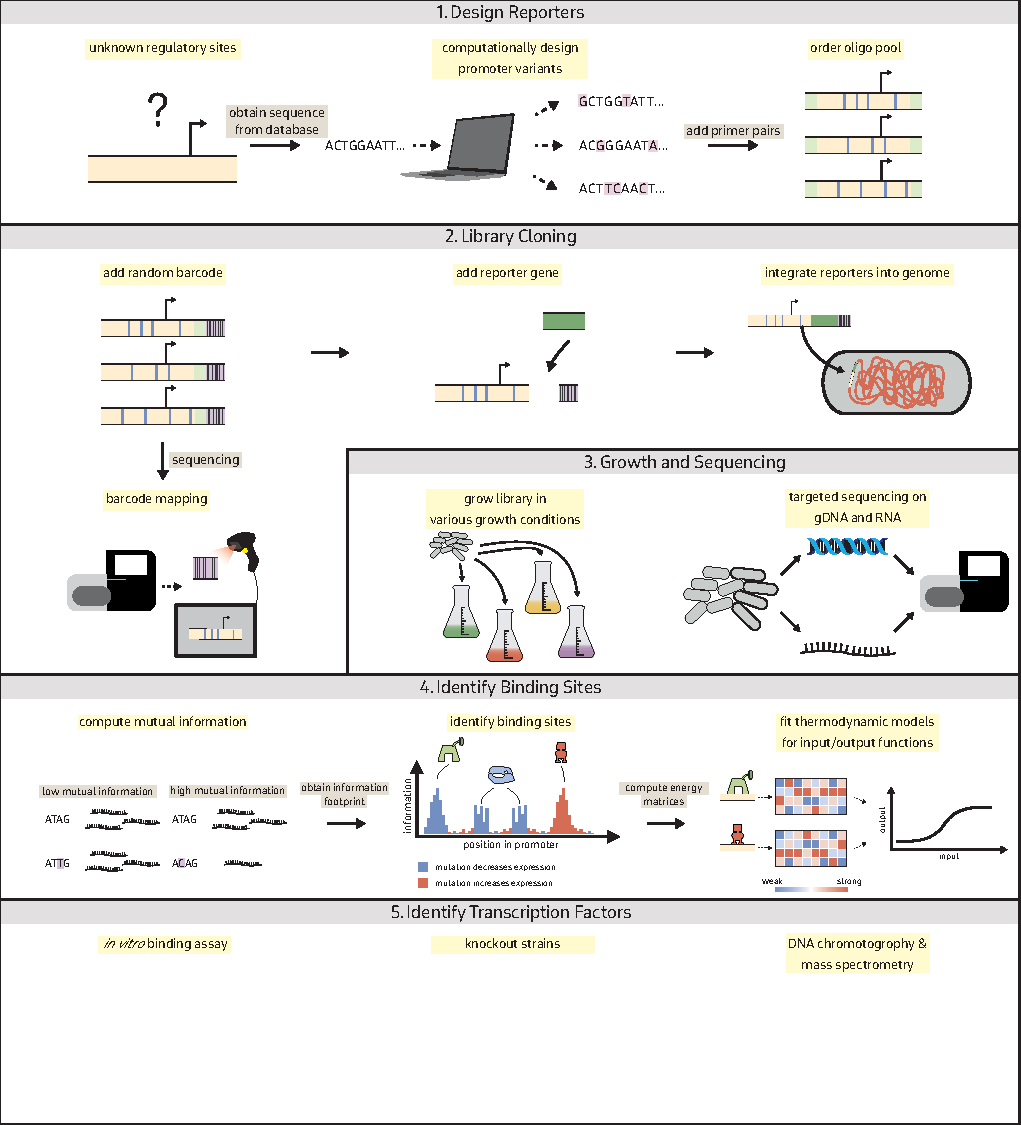
\includegraphics{../figures/figure2_method_sum.pdf}
    \caption{Method summary}
    \label{fig:method_sum}
\end{figure}

\subsection{Genes studied}
104 genes were chosen for this study. 16 of these genes were chosen as so called ``gold standards". These genes have well annotated promoters and have been studied in detail in previous experiments \cite{belliveau2018systematic,ireland2020deciphering}. Including this set of genes allows us to compare the method presented in this work to previous iterations and verify the results, as well as find possible derivations or improvements. 18 genes were chosen that have been identified to have a high variation in protein copy number across a set of 22 growth conditions by Schmidt et al., 2016 \cite{schmidt2016quantitative}. These genes were chosen since a high variation in copy number suggests that there are regulatory proteins controlling the expression of the gene. Of these 18 genes, 9 had no function annotated at the time of this study. Another set of 13 genes was chosen from EcoCyc as part of the so-called y-ome\cite{ghatak2019ome}, which is made up of genes not having any functional annotation. 18 genes were chosen for being part of toxin/anti-toxin systems. Two sets of genes were chosen from the work of Lamoureux et al.\cite{lamoureux2021precise}, where groups of genes which are controlled by the same transcription factor are identified, so called iModulons. We chose two newly identifed groups, responding to the putative transcription factors YmfT and YgeV respectively. Finally, 6 genes were chosen for being part of gene regulatory networks with feed-forward-loop motifs. An entire list of genes can be found in \tr{some SI table}.


\subsection{Barcode Mapping}
For each gene studied here, we designed a library of 1500 mutated promoter variants with an average mutation rate of 0.1 for each promoter that was identified with the gene in EcoCyc. If a gene did not have a promoter identified, we first looked for a possible TSS identified by Urtecho et al., 2018 \cite{urtecho2018systematic}, which then was taken as initial sequence for generating mutated variants. In some cases, no TSS could be identified and we used the model of LaFleur et al., 2022 \cite{lafleur2022automated}, which predicts trancsription start sites for $\sigma^{70}$ promoters given a genomic sequence of \textit{E. coli}, to find the site in the intergenic region leading up to the first coding region in the operon the gene was part of that had the highes predicit affinity for $\sigma70$-factors. A total of 178619 sequences were ordered from Twist Biosciences (1500 mutated variants and wildtype sequence for 119 promoters). Random barcodes were added to the sequences by PCR and they were cloned into a plasmid vector for amplification and subsequent cloning steps . Details can be found in Supplementary information sections \ref{sec:ident_tss}, \ref{sec:comp_prom_muta}, \ref{sec:library_cloning} and  \ref{sec:barcode_mapping}. 171591 ($>$96\%) of sequences were identified in the plasmid library, and an additional 101 sequences were found, likely due to errors in the synthesis process of the oligonucleotide library. For seven genes, there were two TSSs annotated to the same position, likely by TSSs for different sigma factors. For five promoters (tnaCp, crpp1, lpp, yqaEp, dicCp) significantly less variants were recovered. Four of these (tnaCp, crpp1, lpp, yqaEp) have high AT content and thymine repeats in the beginning of the promoter sequence, possibly leading to increased error rates in sequencing \tr{look this up}.
For dicCp, the recovered promoter variants have an increased mutation rate between bases -7 and 12 relative to the TSS, as shown in Fig.~2(B). Is region is exactly the binding site identified for the transcription factor DicA in this promoter \cite{yun2012cnuk9e}. An increased mutation rate indicates that the binding affinity for the transcription factor DicA has to be reduced significantly, indicating that binding of DicA to its functional targets in the genome is essential for growth. CRISPR interference TF knockdown experiments have shown similar lethal effects when targeting DicA\cite{han2023genome}.


\begin{figure}
    \centering
    \includegraphics{../figures/mapping_results.pdf}
    \caption{(A) Recovered promoter variants in barcode mapping. Average mutation rate per base across all promoter variants for galEp1 (B) and dicCp(C). }
    \label{fig:mapping_results}
\end{figure}

\subsection{Expression measurements in 37 growth conditions}




\subsection{Transcription Factor identification}
\subsection{Growth Conditions}
\subsection{Gold Standard genes}
\subsection{Ethanol iModulon}
YgeV has been predicted to be a regulator involved in purine catabolism, leading to the production of allantoin, which can be used as a sole nitrogen source \cite{iwadate2019identification}. There are 16 putative regulatory targets \cite{lamoureux2021precise} for YgeV, including the \textit{xdhABC} operon, which degrades xanthine to uric acid \cite{iwadate2019identification} in the purine catabolism pathway. \textit{E. coli} can survive exposure to low ethanol concentrations up to 5\%, which can even lead to increased DNA synthesis \cite{basu1994effect}, but mostly leads to varies stress responses such as an increased production of ROS. Growth in media supplemented with ethanol induced a change in gene expression for genes regulated by YgeV in a \textDelta\textit{baeR} or \textDelta\textit{cpxR} mutant strain. \tr{Is there a correlation between ethanol response and higher need for nitrogen?}
\subsection{Oxidative stress response iModulon}
The putative transcription factor YmfT regulates 14 out of 23 genes in the e14 prophage and is predicted to respond to oxidative stress \cite{lamoureux2021precise}. Oxidative stress is caused by reactive oxygen species (ROS) such as $\text{H}_2\text{O}_2$, which are highly reactive and damage DNA, the cell wall, proteins \cite{ezraty2017oxidative} etc., however, oxidized amino acids can also lead to confirmational changes in transcription factors, such as OxyR and HypT, which induce DNA binding and subsequent regulation of genes involved in response to oxidative stress  \cite{ezraty2017oxidative}. Hydrogen peroxide is produced endogenously in various pathways in \textit{E. coli} and especially in high amounts when phenylethylamine is used as either carbon or nitrogen source \cite{ravindra2013escherichia}, hence we used used minimal media supplemented with 10 mM 2-phenylethylamine hydrochloride (PEA) as sole carbon source to induce stress responses to $\text{H}_2\text{O}_2$ and therefore oxidative stress. \tr{discuss findings of ymfT modulon and how it relates to oxyR, look at oxyR iModulons and possibly do another run including this gene.}
\subsection{Antitoxin/Antibiotic genes}
\subsection{other y-ome genes}
